\documentclass{atistandalonetask}
\usepackage{atistandard}
\begin{document}
  \begin{atiTask}[
    title = Delta- und Heaviside-Distributionen
  ]
  
 \begin{atiSubtasks}
 \item Berechnen Sie die folgenden Integrale:
 	\begin{atiSubequations}
 	\item{\integral{0}{2,8}{\delta(x-e)\ln x}{x}}
 	\item{\integral{0}{\infty}{\frac{e^x}{x^2}\delta(x+1)}{x}}
 	\item{\integral{-\infty}{\infty}{x\delta(x)(a_0+a_1x+a_2x^2+a_3x^3)}{x}}
 	\item{\integral{-\infty}{2\pi}{\cos x\delta(x^2-\pi^2)}{x}}
 	\end{atiSubequations}
 \item Stellen Sie die Ladungsverteilung $\rho(x,y)$ zu folgender Skizze, bestehend aus 4 Punktladungen und einer Linienladung, auf. 
\begin{figure}[H]
\centering
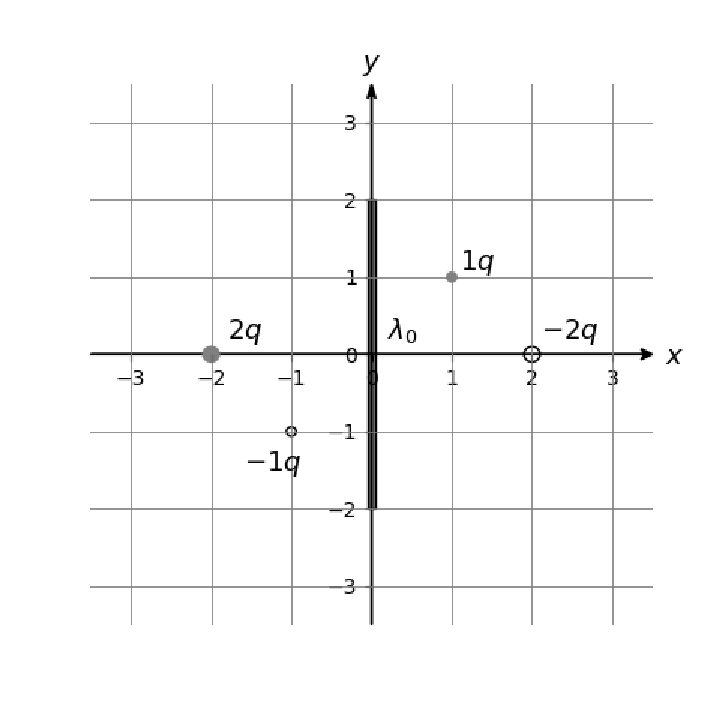
\includegraphics[width=0.6\linewidth]{picture-delta_vii.pdf}
\end{figure}
 
 \item Skizzieren Sie die folgende Funktion:
 \[
 g(x)=-x\Theta(-x)\Theta(x+1)-(x-3)\Theta(x-2)\Theta(3-x)+\frac{x}{2}\Theta(2-x)\Theta(x).
 \]
 \end{atiSubtasks}

  \end{atiTask}
  \begin{atiSolution}
Loesung folgt
  %	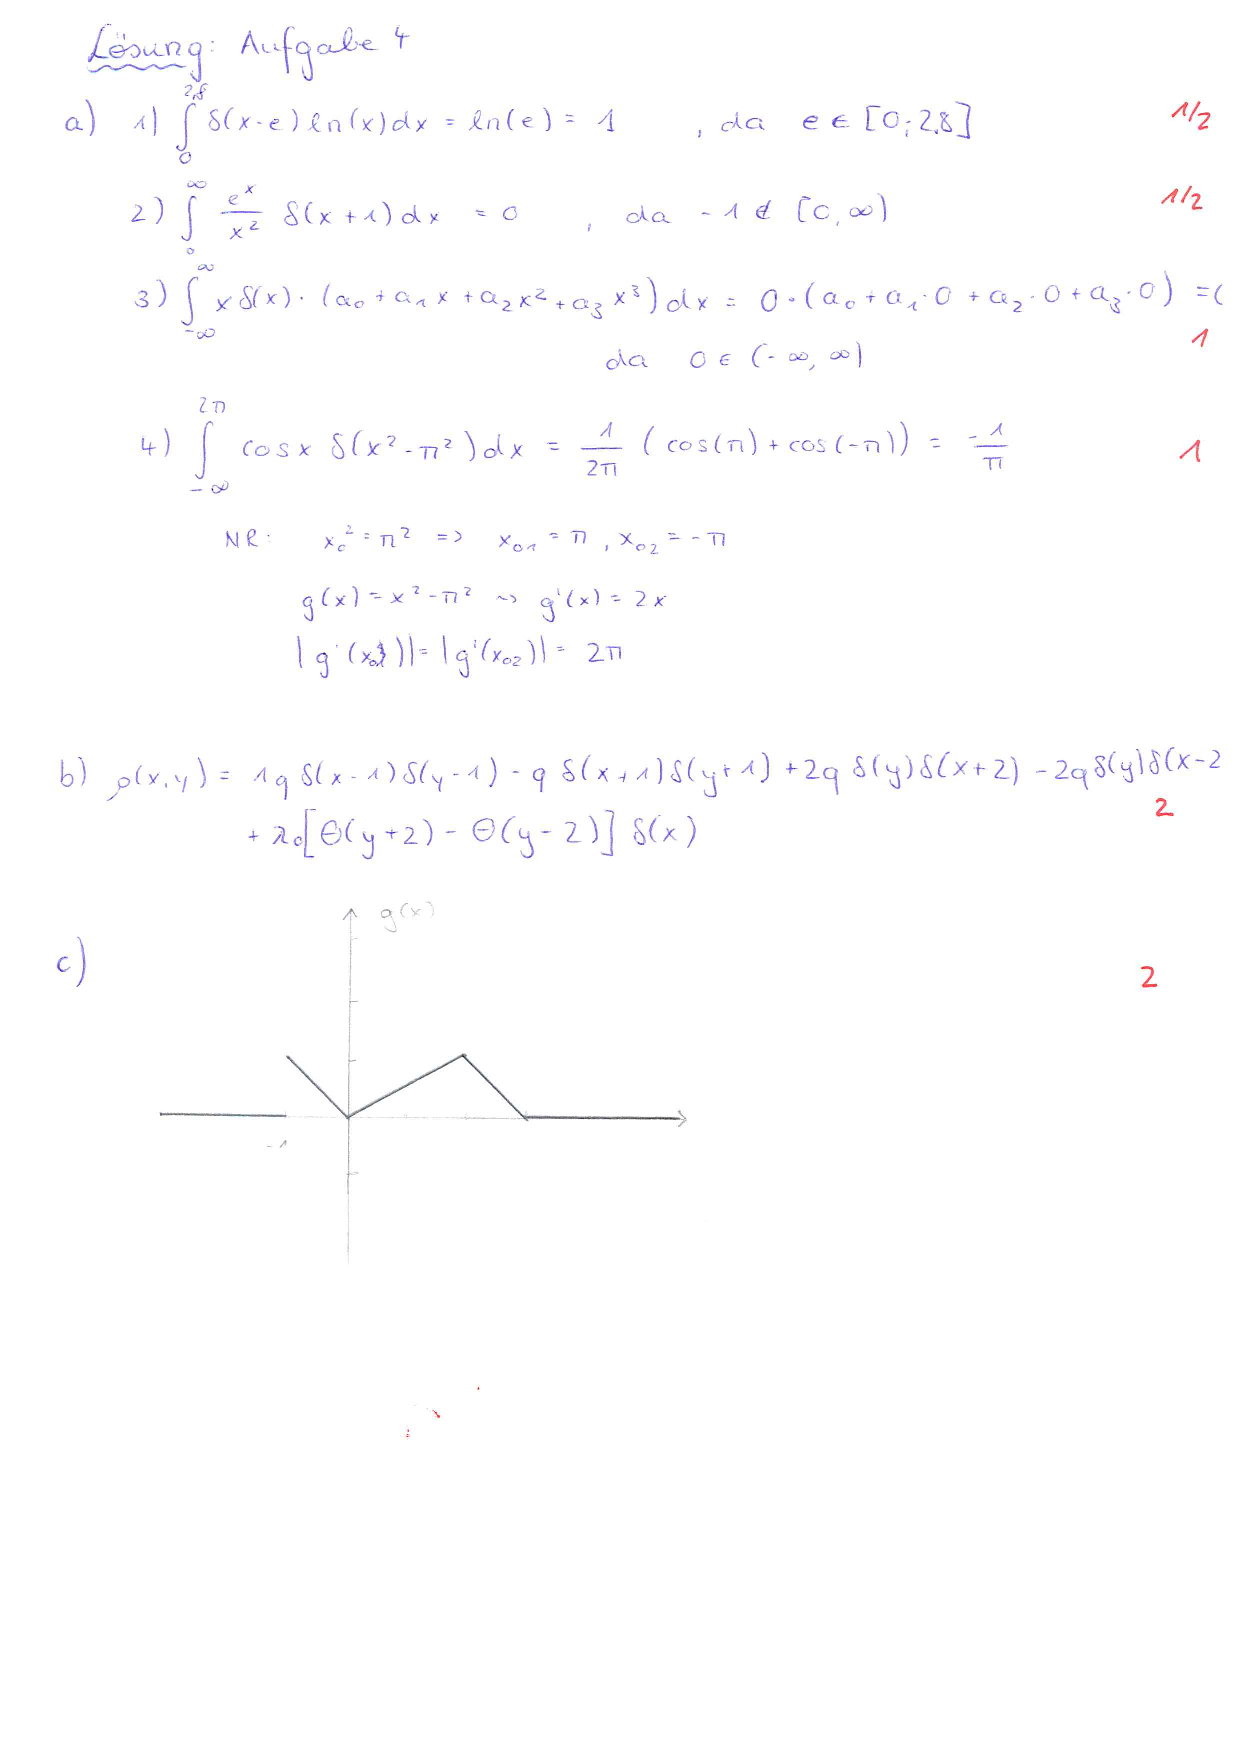
\includepdf[pages=-]{solution-delta_vii.pdf}
  \end{atiSolution}
\end{document}